\documentclass[8pt]{article}

% Packages
\usepackage[a4paper,margin=0.8in]{geometry}
\usepackage{graphicx}
\usepackage{multicol}
\usepackage{xcolor}
\usepackage{helvet}
\renewcommand{\familydefault}{\sfdefault}

\usepackage{hyperref} % Required for adding links	and customizing them
\definecolor{linkcolour}{rgb}{0,0.2,0.6} % Link color
\hypersetup{colorlinks,breaklinks,urlcolor=linkcolour,linkcolor=linkcolour} % Set link colors throughout the document

\newcommand{\faqurl}{https://tr.ee/gwfaq}
\newcommand{\obsegg}{https://www.linkedin.com/posts/lugano-plan-b_luganoplanb-bitcoin-activity-7167881837728493568-LEZk/}
\newcommand{\theproblem}{https://x.com/search?q=jameson\%20lopp\%20wrench\%20attack&src=typed_query&f=live}
\newcommand{\nocurrentsolution}{https://www.youtube.com/watch?v=MsfR6ZIkzPs&t=2734s}
\newcommand{\kba}{https://en.wikipedia.org/wiki/Knowledge-based_authentication}
\newcommand{\kprinciple}{https://en.wikipedia.org/wiki/Kerckhoffs's_principle}
\newcommand{\privsecplaque}{https://duckduckgo.com/?q=prosegur+verisure+\%22warning+sign\%22+facade\&iar=images\&t=brave\&iaf=type\%3Aphoto}

% Colors
\definecolor{accent}{RGB}{247, 147, 26}

% Custom Commands
\newcommand{\feature}[2]{
    \noindent\textbf{\large #1}\par
    \vspace{2pt}
    #2
    \vspace{11pt}
}

% Document
\begin{document}
\pagestyle{empty}  % <-- disables all page numbering
% Title Section
\begin{center}
    \vspace*{-1cm}
    {\huge\bfseries\color{accent} Great Wall: Reinventing Coercion-Resistance}\\[1ex]
    {\large\textit{``I have never seen an unworried Bitcoiner''}}
    \vspace{0.2cm}
\end{center}

% App Description
\noindent
The 2023-2026 Bitcoin cycle has been witnessing a \href{\theproblem}{terrifying rise in the frequency and gravity of \textbf{wrench attacks}} (theft of crypto assets through robbery or kidnapping), and, \href{\nocurrentsolution}{embarrassingly, crypto community doesn't have a simple, effective and affordable solution for it}. Yet. Meet \textbf{Great Wall}, an innovative self-custody protocol for coercion-resistance. It is \textbf{the only} to combine the following four properties below: 

\vspace{0.2cm}

% Features Section
{\color{accent}\hrule}
\vspace{0.2cm}
{\Large\textbf{Key Features}}
\vspace{0.2cm}
{\color{accent}\hrule}
\vspace{0.2cm}

\begin{multicols}{2}
    \feature{1 \href{\kba}{Deviceless / KBA}}{
        No gadget, metal plate, vault, physical address, etc (additional points of failure) are necessary for the key derivation. 
    }

    \feature{2 Non-Shared Custody}{
        You don't compromise Bitcoin's foundational premise of \textbf{individual} custody.
    }

    \feature{3 \href{\kprinciple}{Non-Obscurity}}{
        You don't need to \href{\obsegg}{hide in shadows}, nor wish on your lucky start that your secret trick (like decoy wallet) is never learned by the bad guys.
    }

    \feature{4 Coercion-Resistance}{
        Commitment or threat of violence on user yields no material benefit to the attacker in any circumstance.
    }
\end{multicols}

% \vspace{0.5cm}

% Features Section
{\color{accent}\hrule}
\vspace{0.2cm}
{\Large\textbf{How It Works}}
\vspace{0.2cm}
{\color{accent}\hrule}
\vspace{0.3cm}

\noindent
Simply put: ``1) It's all in your brain; 2) in nobody else's; 3) the attacker knows about it; and 4) they are, nevertheless, unable to coerce you into giving away your keys''. Let's see how to deliver all that, and 5) monetize it!

% Visual / Screenshot (optional)
\begin{center}
    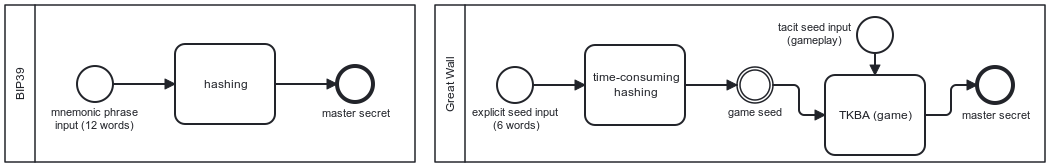
\includegraphics[width=1\textwidth]{gw-one-pager-diagram.png}
    \textit{Comparative BPMN diagrams representing BIP39 and Great Wall key derivation schemes.}
\end{center}

\noindent
Likewise BIP39, it's just a key derivation scheme that can run 100\% offline in any device. The simple way to describe the Great Wall protocol is to say:

\begin{enumerate}
 \item You input an initial seed equivalent in strength to 6 BIP39 words into an \href{\faqurl}{hours-long hash};
 \item Hash specifies a seed to your `private game', which admits a near-infinity of possible `gameplays';
 \item Bits of your `private gameplay' of your `private game' are added to the entropy of the master secret;
\end{enumerate}

\noindent
The catch is that the knowledge of `gameplay' is easy to memorize but impossible to put into words. Because of that, you, kept alive and well, are strictly necessary during the entire process, \href{\faqurl}{which can be set up to take hours, days, or even weeks}. As a result, stealing your stash becomes at least as difficult as conducting a kidnapping that takes as long. Similarly to \href{https://apps.ankiweb.net/}{Anki} and \href{https://www.duolingo.com/}{Duolingo}, an \textbf{integrated memory coach} prevents user \textit{forgetting} their seeds due to \textit{insufficiently} exercising brain memory of them; but also user \textit{fatigue} due to \textit{overdoing} it. Replaying this half minute game-like UX on average once a week comfortably cements your lifelong coercion-resistant access to your stash.

\vspace{0.3cm}

{\color{accent}\hrule}
\vspace{0.2cm}
{\Large\textbf{Monetization} --- \href{\faqurl}{first-mover lock-in}}
\vspace{0.2cm}
{\color{accent}\hrule}
\vspace{0.3cm}

% The following are revenue streams with first-mover advantage and natural market consolidation:
\begin{enumerate}
 \item \textbf{branded merchandise} --- likewise \href{\privsecplaque}{security companies' warning signs}, it dissuades would-be wrench attackers and propagate virally;
 \item \textbf{convenience} --- for a small price, \href{\faqurl}{without compromise of security properties}, you can choose to outsource the hours-, days- or weeks-long inconvenience of keeping your own device very busy;
 \item \textbf{hardware} --- for premium UX, high-end users will prefer dedicated air gapped hardware;
 \item \textbf{inheritance protocol} --- same market and similar mechanism to 2, also recurrent micropayment;
\end{enumerate}

% Call to Action

\noindent
{\color{accent}\rule{\linewidth}{0.5mm}}
% \vspace{0.1cm}
\begin{center}
%     {\Large\textbf{Available now on [Platforms]!}}\\
Visit \href{https://linktr.ee/greatwallt3}{linktr.ee/greatwallt3} to verify all claims and learn more.
\end{center}

\end{document}
